\documentclass{article}

% Language setting
% Replace `english' with e.g. `spanish' to change the document language
\usepackage[english]{babel}

% Set page size and margins
% Replace `letterpaper' with`a4paper' for UK/EU standard size
\usepackage[letterpaper,top=2cm,bottom=2cm,left=3cm,right=3cm,marginparwidth=1.75cm]{geometry}

% Useful packages
\usepackage{amsmath}
\usepackage{graphicx}
\usepackage[colorlinks=true, allcolors=blue]{hyperref}

\title{Esercizio 4}
\author{Ruben Castelluccio}

\begin{document}
\maketitle

\section{Introduzione}
L'esercizio 4 consiste nella verifica delle proprietà in diverse varianti a partire dall'algoritmo 3.2 per la mutua esclusione fino all'algoritmo 3.10 denominato Algoritmo di Dekker. Si richiede di definire gli algoritmi mediante l'utilizzo di:
\begin{itemize}
    \item GreatSPN: per la definizione della rete di Petri, la costruzione del RG e la verifica delle proprietà richieste;
    \item Algebra dei Processi: per i primi 2 algoritmi (3.2. e 3.6) è richiesta la costruzione del DG;
    \item NuSMV: implementazione di tutti gli algoritmi e verifica delle proprietà mediante LTL e CTL.
\end{itemize}
Inoltre per tutti gli algoritmi si verificano:
\begin{itemize}
    \item MUTUA ESCLUSIONE: le istruzioni delle sezioni critiche di due o piu` processi non possono essere eseguite in modo interfogliato;
    \item DEADLOCK: Se qualche processo cerca di accedere alla regione critica eventualmente un processo potrà farlo;
    \item STARVATION: Se un processo cerca di accedere alla regione critica eventualmente quel processo potra’ farlo.
\end{itemize}
Inoltre per gli algoritmi 3.2 e 3.6,in cui è richiesto di riportare il Reachability Graph, si nota che NuSMV, mediante il comando \textit{print\_reachable\_states -v}, costruisce un numero di stati raggiungibili esattamente pari al numero ottenuto nel RG per le reti PT. In particolare nell'algoritmo 3.2 si hanno 16 stati mentre nell'algoritmo 3.6  si ottengono 25 stati.
\clearpage
\section{Algoritmo 3.2}
L'algoritmo 3.2 prevede una variabile di turno \textit{turn} che viene modificata al termine della regione critica di ogni processo in modo da permettere l'esecuzione dell'altro processo. L'algoritmo prevede che ogni processo, all'inizio della propria esecuzione, possa senza limiti ciclare in sezione non critica bloccando l'altro processo. 
\begin{figure}[h] 
\centering
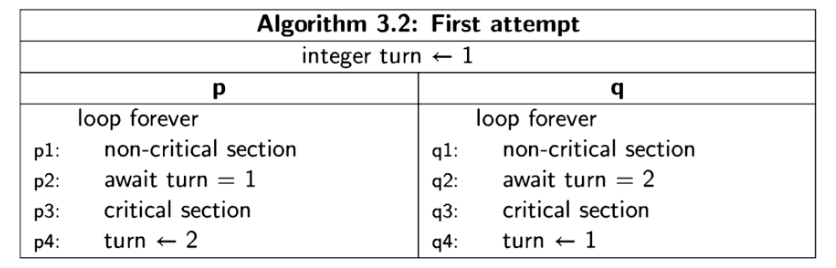
\includegraphics[scale=0.6]{3.2.png}
\end{figure}
\clearpage
\subsection{Rete di Petri}
\begin{figure}[h] 
\centering
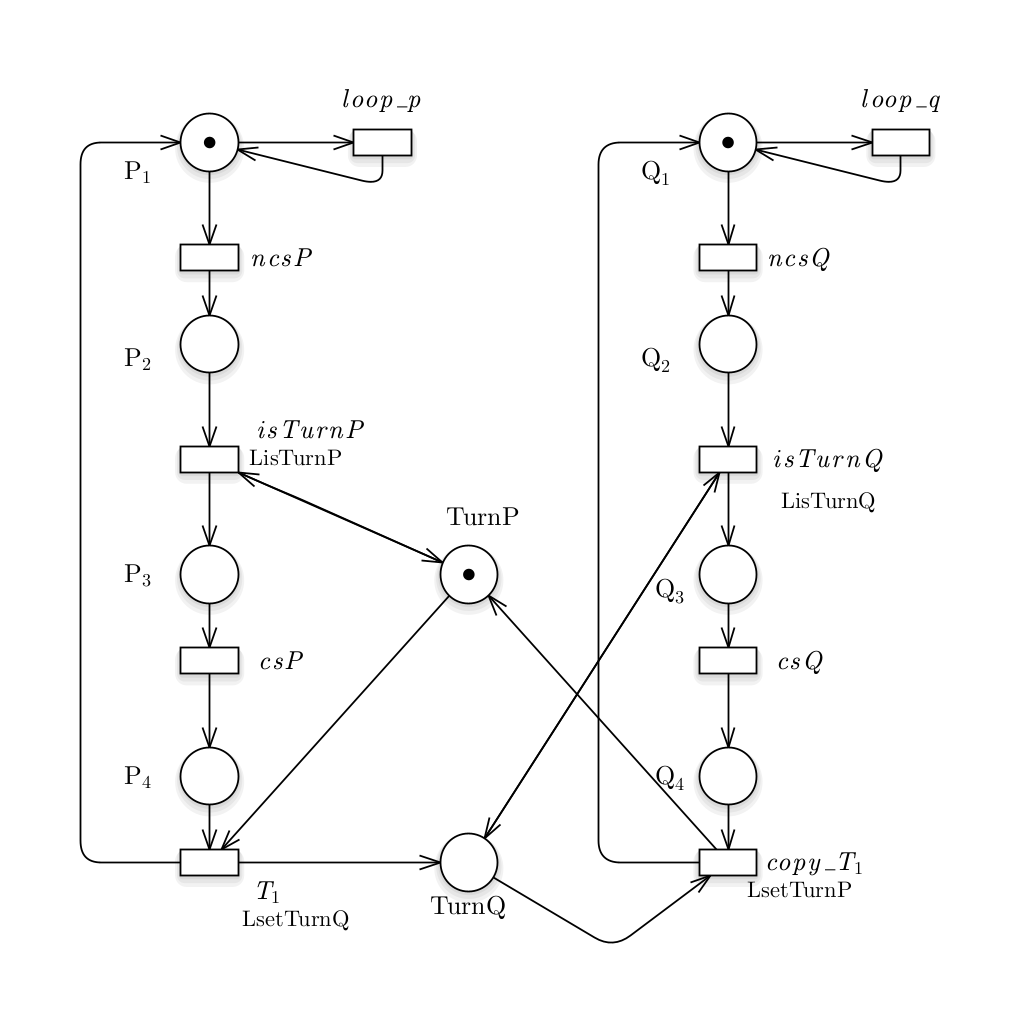
\includegraphics[scale=0.5]{3.2PT.png}
\end{figure}
\subsection{Analisi GreatSPN}
\begin{tabular}{ |p{6cm}||p{3cm}|p{3cm}|}
 \hline
 PROPRIETA'& CTL\\
 \hline
 MUTUA ESCLUSIONE&TRUE \\
 DEADLOCK PROCESSO p&FALSE \\
 DEADLOCK PROCESSO q&FALSE\\
 STARVATION PROCESSO p&FALSE\\
 STARVATION PROCESSO p&FALSE\\
\hline
\end{tabular}
\begin{itemize}
    \item MUTUA ESCLUSIONE: è rispettata in quanto i processi non posso trovarsi contemporaneamente in sezione critica.
    \item DEADLOCK: non è rispettato in quanto i processi posso rimanere all'infinito in regione non critica (p1 e q1) essendo che non sono obbligati al progresso;
    \item STARVATION: non è rispettata in quanto c'è deadlock.
\end{itemize}
\clearpage
\subsection{Reachability Graph}
\begin{figure}[h] 
\centering
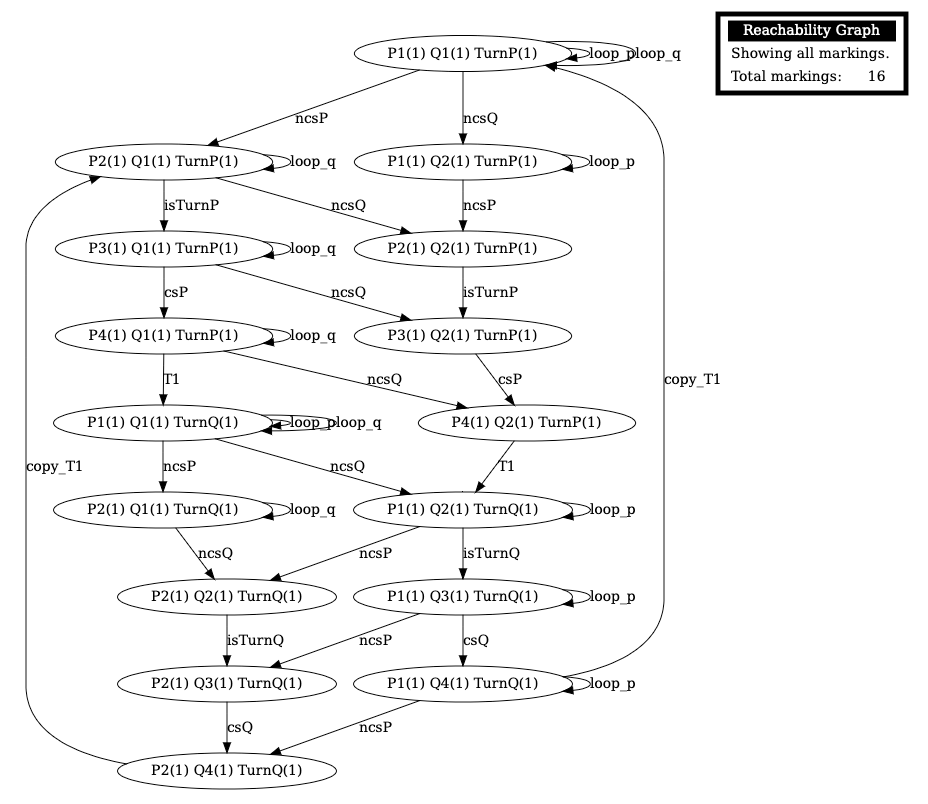
\includegraphics[scale=0.55]{RG3.2.png}
\end{figure}
\clearpage
\subsection{Algebra di Processi - CSP}
In Algebra dei Processi sono definiti 2 processi distinti \textit{p} e \textit{q} che eseguono azioni locali \textit{ncsP1, ncsP} e \textit{ncsQ1} e azioni che richiedono la sincronizzazione con \textit{turn} in modo da ottenere l'ingresso in sezione critica in mutua esclusione e cambiandone il valore all'uscita da quest'ultima. Inoltre i processi possono ciclare in sezione non critica mediante l'azione locale \textit{ncsP1} e \textit{ncsQ1}.
\\\\s = \{isP, isQ, setP, setQ\}
\\TurnP = isP.TurnP + setP.TurnP + setQ.TurnQ
\\TurnQ = isQ.TurnQ + setQ.TurnQ + setP.TurnP
\\
\\P1 = ncsP1.P1 + ncsP2.P2 
\\P2 = isP.P3
\\P3 = csP.P4
\\P4 = setQ.P1
\\
\\Q1 = ncspQ1.Q1 + ncspQ2.Q2
\\Q2 = isQ.Q3
\\Q3 = csQ.Q4
\\Q4 = setP.Q1
\begin{figure}[h] 
\centering
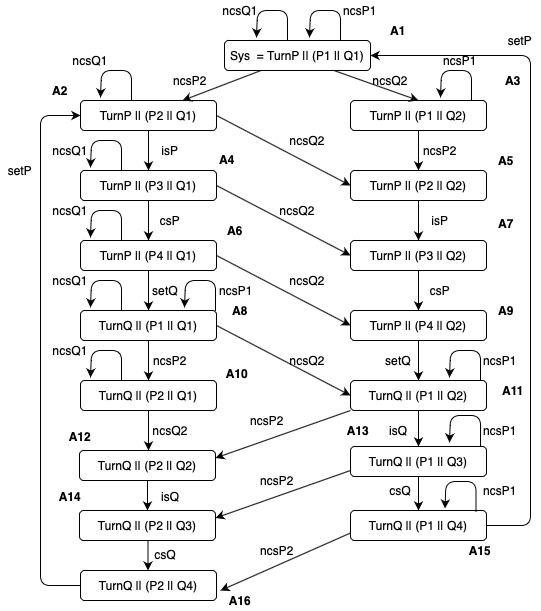
\includegraphics[scale=0.7]{DG3.2.png}
\end{figure}
\subsection{Confronto tra Reachability Graph vs Derivation Graph}
Dal confronto tra il Reachability Graph ottenuto dalla rete di Petri tramite GreatSPN e il Derivation Graph ottenuto dall'algebra dei processi si evidenzia la corrispondenza nel numero di stati presenti (16). 
\clearpage
\subsection{NuSMV}
L'implementazione dell'algoritmo 3.2 in NuSMV prevede un modulo main in cui si definisce una variabile globale \textit{turn} e 2 processi \textit{p} e \textit{q} mediante il modulo user che ha come parametri la stessa variabile \textit{turn} e 2 valori che rappresentano rispettivamente il valore della variabile \textit{turn} rispetto al processo in esecuzione. 
\\Nel modulo user sono definiti 4 stati in maniera analoga a quanto fatto dall'algoritmo 3.2:
\begin{itemize}
    \item p1 : esecuzione in regione non critica;
    \item p2 : in attesa che la variabile \textit{turn} sia pari al valore di \textit{myproc};
    \item p3 : esecuzione in regione critica
    \item p4 : uscita dalla regione critica e variabile \textit{turn} impostata al valore della varibile \textit{otherproc}.
\end{itemize}
\begin{figure}[h] 
\centering
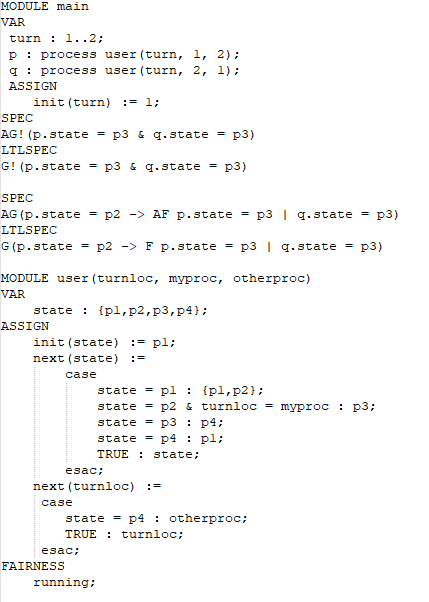
\includegraphics[scale=1.1]{3.2nusmv.png}
\end{figure}
\subsection{Analisi NuSMV LTL}
MUTUA ESCLUSIONE:
\\LTLSPEC
\\G!(p.state = p3 \& q.state = p3)
\\\\DEADLOCK DEL PROCESSO p:
\\LTLSPEC
\\G(p.state = p2 -$>$ F p.state = p3 $|$ q.state = p3)
\\\\DEADLOCK DEL PROCESSO q:
\\LTLSPEC
\\G(q.state = p2 -$>$ F p.state = p3 $|$ q.state = p3)
\\\\STARVATION DEL PROCESSO p:
\\LTLSPEC
\\G(p.state = p2 -$>$ F p.state = p3)
\\\\STARVATION DEL PROCESSO q:
\\LTLSPEC
\\G(q.state = p2 -$>$ F q.state = p3)
\subsection{Analisi NuSMV CTL}
MUTUA ESCLUSIONE
\\SPEC
\\G!(p.state = p3 \& q.state = p3)
\\\\DEADLOCK DEL PROCESSO p:
\\SPEC
\\AG(p.state = p2 -$>$ AF p.state = p3 $|$ q.state = p3)
\\\\DEADLOCK DEL PROCESSO q:
\\SPEC
\\AG(q.state = p2 -$>$ AF p.state = p3 $|$ q.state = p3)
\\\\STARVATION DEL PROCESSO p:
\\SPEC
\\AG(p.state = p2 -$>$ AF p.state = p3)
\\\\STARVATION DEL PROCESSO q:
\\SPEC
\\AG(q.state = p2 -$>$ AF q.state = p3)
\subsection{Analisi Proprietà NuSMV}
\begin{tabular}{ |p{6cm}||p{3cm}|p{3cm}|}
 \hline
 PROPRIETA' & LTL & CTL\\
 \hline
 MUTUA ESCLUSIONE&TRUE&TRUE \\
 DEADLOCK PROCESSO p&FALSE&FALSE \\
 DEADLOCK PROCESSO q&FALSE&FALSE \\
 STARVATION PROCESSO p&FALSE&FALSE\\
 STARVATION PROCESSO p&FALSE&FALSE\\
\hline
\end{tabular}
\begin{itemize}
    \item MUTUA ESCLUSIONE: è rispettata in quanto la variabile turn, condivisa da entrambi i processi, impedisce che possano accedere in regione critica contemporaneamente .
    \item DEADLOCK: non è rispettato in quanto i processi posso ciclare all'infinito in regione non critica (p1 e q1) essendo che non sono obbligati al progresso, nel contro esempio fornito da NuSMV si osserva come in maniera speculare i processi \textit{p} e \textit{q} potrebbero esere in attesa che la variabile condivisa \textit{turn} sia settata ad un valore tale da permettere l'accesso in regione critica ma questo non accade in quanto l'altro processo esegue infinitamente spesso la regione non critica \textit{p1} non modificando la variabile condivisa.
    \item STARVATION: non è rispetta in quanto non c'è assenza di deadlock.
\end{itemize}
\clearpage
\section{Algoritmo 3.6}     
L'algoritmo 3.6 prevede 2 variabili boolean \textit{wantp} e \textit{wantq} che vengono impostate rispettivamente a \textit{true} nel processo \textit{p} e \textit{q} per poter entrare nella regione critica e al termine al fine di permettere l'esecuzione dell'altro processo settando a \textit{false}. L'algoritmo prevede che ogni processo, all'inizio della propria esecuzione, possa senza limiti ciclare in sezione non critica bloccando l'altro processo. 
\begin{figure}[h] 
\centering
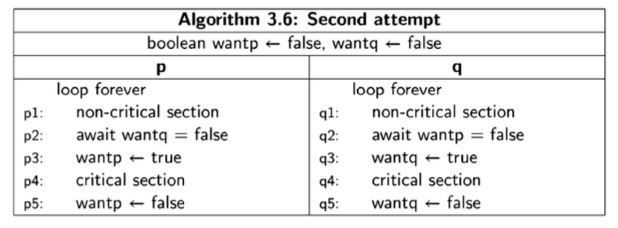
\includegraphics[scale=0.6]{3.6.png}
\end{figure}
\clearpage
\subsection{Rete di Petri}
\begin{figure}[h] 
\centering
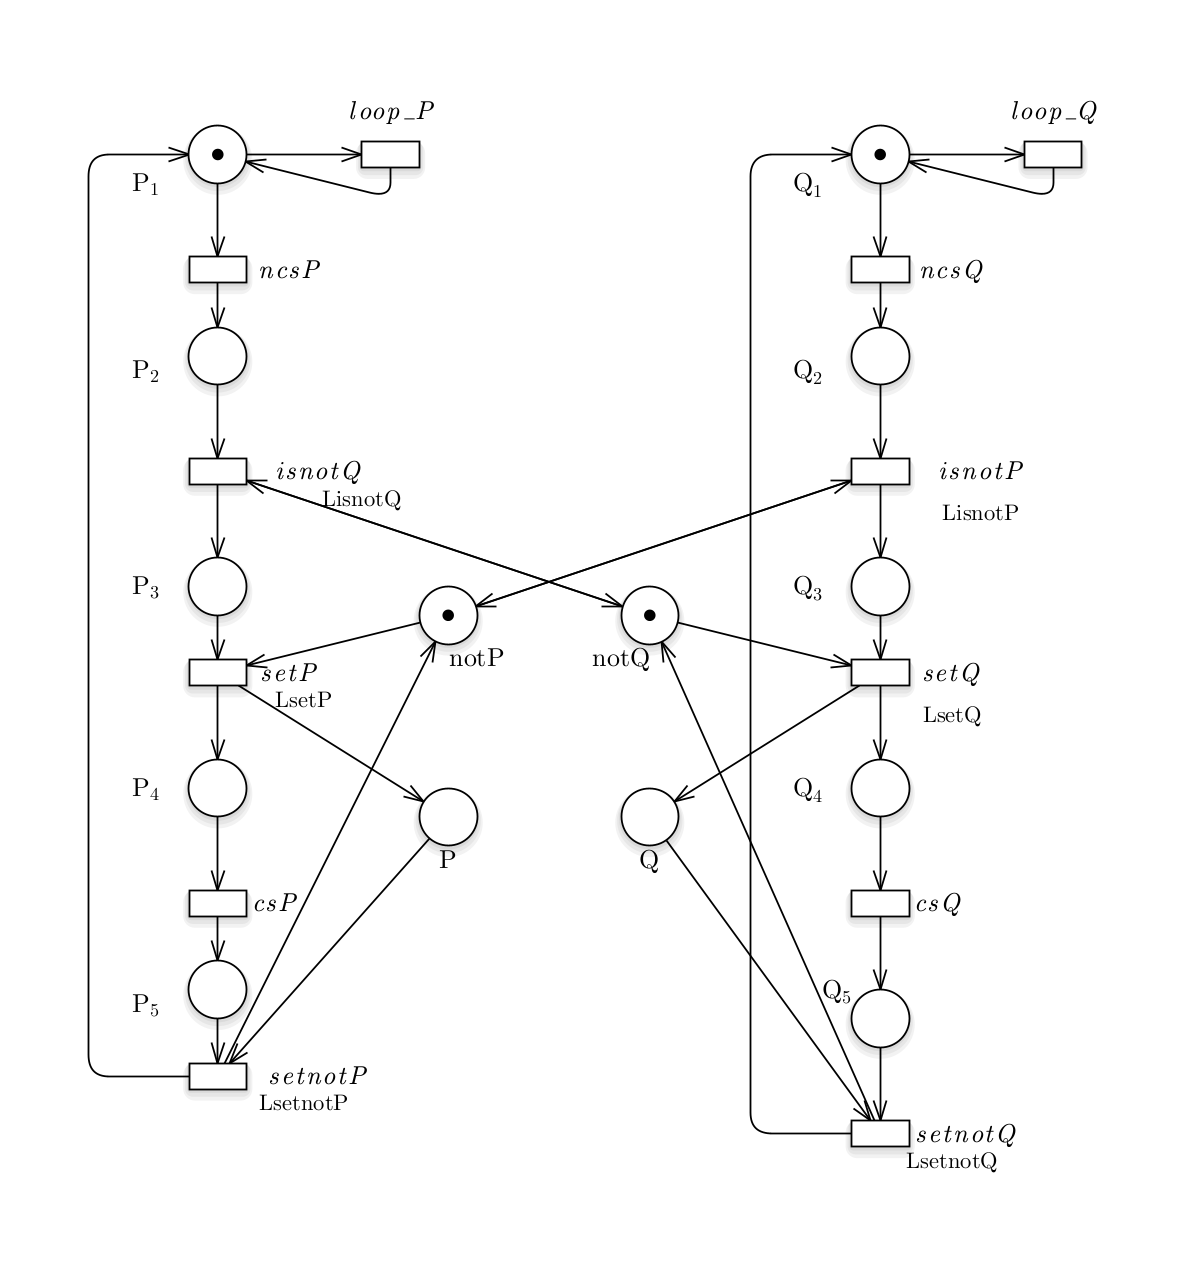
\includegraphics[scale=0.4]{3.6-5.png}
\end{figure}
\subsection{Analisi GreatSPN}
\begin{tabular}{ |p{6cm}||p{3cm}|p{3cm}|}
 \hline
 PROPRIETA'& CTL\\
 \hline
 MUTUA ESCLUSIONE&FALSE \\
 DEADLOCK PROCESSO p&FALSE \\
 DEADLOCK PROCESSO q&FALSE\\
 STARVATION PROCESSO p&FALSE\\
 STARVATION PROCESSO p&FALSE\\
\hline
\end{tabular}
\begin{itemize}
    \item MUTUA ESCLUSIONE: non è rispettata in quanto è possibile che entrambi i processi si trovino contemporaneamente in regione critica dato che le verifiche \textit{isnotQ} e \textit{isnotP} e successivamente \textit{setP} e \textit{setQ} non impediscono che questa situazione si crei, come riportato dal contro esempio di NuSMV può accadere che i processi \textit{p} e \textit{q} avanzino insieme ed entrando in regione critica.
    \item DEADLOCK: non è rispettato in quanto i processi posso ciclare all'infinito in regione non critica (p1 e q1) essendo che non sono obbligati i processi al progresso;
    \item STARVATION: non è rispettata in quanto non c'è assenza di deadlock.
\end{itemize}
\clearpage
\subsection{Reachability Graph}
\begin{figure}[h] 
\centering
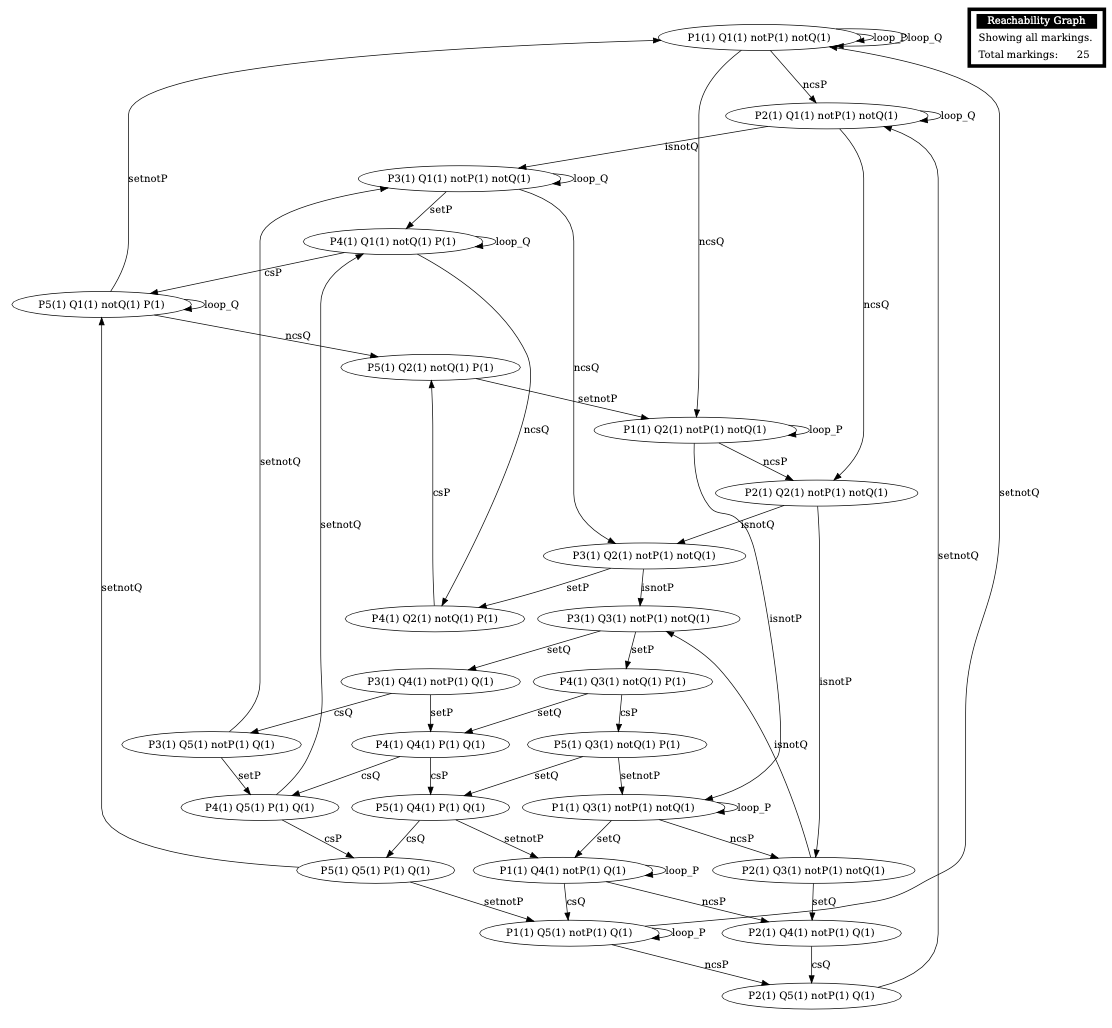
\includegraphics[scale=0.45]{RG3.6.png}
\end{figure}
\subsection{Algebra di Processi - CSP}
In Algebra dei Processi sono definiti 2 processi distinti \textit{p} e \textit{q} che eseguono azioni locali \textit{ncsP1, ncsP} e \textit{ncsQ1} e azioni che richiedono la sincronizzazione con le variabili \textit{notWantP} e \textit{notWantQ} in modo da verificare sia che la variabile relativa all'altro processo sia settata a false sia che la propria sia true permettendo la sincronizzazione per l'ingresso in sezione critica in mutua esclusione e cambiandone il valore all'uscita da quest'ultima. Inoltre i processi possono ciclare in sezione non critica mediante l'azione locale \textit{ncsP1} e \textit{ncsQ1}.
\\\\s = \{isnotP, isnotQ, setP, setQ, setnotP, setnotQ\}
\\notWantP = setP.WantP + isnotQ.notWantP
\\WantP =  setnotP.WantQ
\\notWantQ = setP.WantQ + isnotP.notWantQ 
\\WantQ = setnotQ.WantP
\\
\\P1 = ncsP1.P1 + ncsP2.P2 
\\P2 = isnotQ.P3
\\P3 = setP.P4
\\P4 = csP.P4
\\P5 = setnotP.P1
\\
\\Q1 = ncspQ1.Q1 + ncspQ2.Q2
\\Q2 = isnotP.Q3
\\Q3 = setQ.Q4
\\Q4 = csQ.Q5
\\Q5 = setnotQ.Q1
\begin{figure}[h] 
\centering
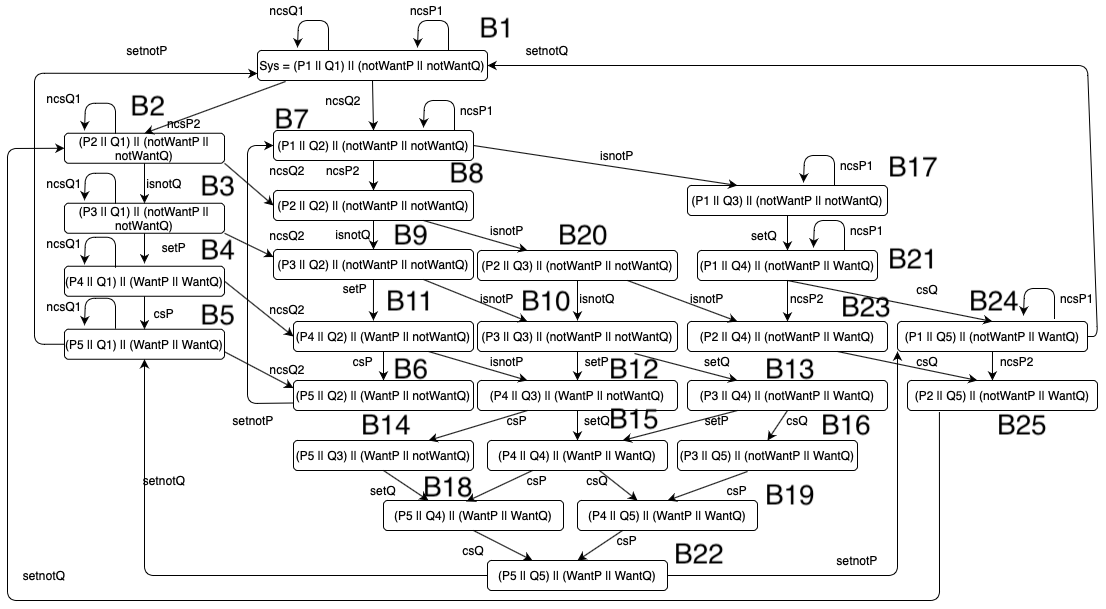
\includegraphics[scale=0.45]{CSP3.6.png}
\end{figure}
\subsection{Confronto tra Reachability Graph vs Derivation Graph}
Analogamente a quanto evidenziato nel confronto dell'algoritmo 3.2 anche in questo viene rilevato una diretta corrispondenza nel numero degli stati (25).
\clearpage
\subsection{NuSMV}
L'implementazione dell'algoritmo 3.6 in NuSMV prevede un modulo main in cui si definiscono 2 variabili di tipo boolean impostate entrambe a FALSE \textit{wantp} e \textit{wantq} e 2 processi \textit{p} e \textit{q} e il modulo user che ha come parametri le variabili  \textit{wantp} e \textit{wantq}. 
\\Nel modulo user sono definiti 5 stati in maniera analoga a quanto fatto dall'algoritmo 3.6:
\begin{itemize}
    \item p1 : esecuzione in regione non critica;
    \item p2 : in attesa che la variabile \textit{wantq} sia FALSE;
    \item p3 : la variabile \textit{wantp} è impostata a TRUE;
    \item p4 : esecuzione in regione critica;
    \item p5 : uscita dalla regione critica e variabile \textit{wantp} impostata a FALSE.
\end{itemize}
\begin{figure}[h] 
\centering
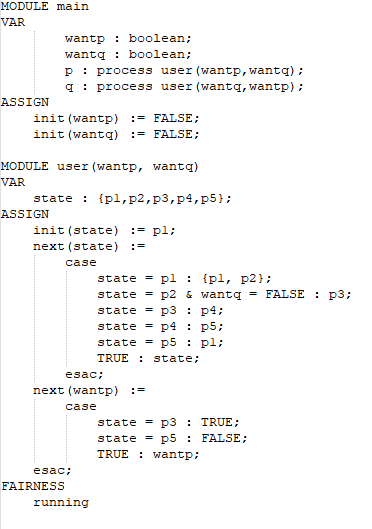
\includegraphics[scale=1.2]{3.6nusmv.png}
\end{figure}
\subsection{Analisi NuSMV LTL}
MUTUA ESCLUSIONE:
\\LTLSPEC
\\G!(p.state = p4 \& q.state = p4)
\\\\DEADLOCK DEL PROCESSO p:
\\LTLSPEC
\\G(p.state = p2 -$>$ F p.state = p4 $|$ q.state = p4)
\\\\DEADLOCK DEL PROCESSO q:
\\LTLSPEC
\\G(q.state = p2 -$>$ F p.state = p4 $|$ q.state = p4)
\\\\STARVATION DEL PROCESSO p:
\\LTLSPEC
\\G(p.state = p2 -$>$ F p.state = p4)
\\\\STARVATION DEL PROCESSO q:
\\LTLSPEC
\\G(q.state = p2 -$>$ F q.state = p4)
\subsection{Analisi NuSMV CTL}
MUTUA ESCLUSIONE
\\SPEC
\\G!(p.state = p4 \& q.state = p4)
\\\\DEADLOCK DEL PROCESSO p:
\\SPEC
\\AG(p.state = p2 -$>$ AF p.state = p4 $|$ q.state = p4)
\\\\DEADLOCK DEL PROCESSO q:
\\SPEC
\\AG(q.state = p2 -$>$ AF p.state = p4 $|$ q.state = p4)
\\\\STARVATION DEL PROCESSO p:
\\SPEC
\\AG(p.state = p2 -$>$ AF p.state = p4)
\\\\STARVATION DEL PROCESSO q:
\\SPEC
\\AG(q.state = p2 -$>$ AF q.state = p4)
\subsection{Analisi Proprietà NuSMV}
\begin{tabular}{|p{6cm}||p{3cm}|p{3cm}|}
\hline
PROPRIETA' & LTL & CTL\\
\hline
 MUTUA ESCLUSIONE&FALSE&FALSE \\
 DEADLOCK PROCESSO p&TRUE&TRUE\\
 DEADLOCK PROCESSO q&TRUE&TRUE \\
 STARVATION PROCESSO p&FALSE&FALSE\\
 STARVATION PROCESSO p&FALSE&FALSE\\
\hline
\end{tabular}
\\
Si noti una differenza sostanziale tra i risultati riportati da NuSMV e GreatSPN a causa del differente concetto di fairness che viene implementato e in particolare in NuSMV la proprietà è specificata da FAIRNESS running e pertanto si considerano solo le esecuzioni in cui le proprietà da verificare risultano infinatamente spesso essere vere.
\begin{itemize}
    \item MUTUA ESCLUSIONE: non è rispetta in quanto, come dimostrato dai controesempi forniti da NuSMV, è possibile che entrambi i processi entrino in regione critica dato che la verifica che la variabile boolean \textit{wantp} o \textit{wantq}, a seconda del processo, sia impostata a FALSE non assicura la mutua esclusione;
    \item DEADLOCK: è rispettato se viene definita la fairness running che impedisce a un processo di non progredire nell'esecuzione;
    \item STARVATION: non è rispettata in quanto un processo potrà eseguire le proprie istruzioni all'infinito impedendo l'accesso all'altro processo.
\end{itemize}
\subsection{Bisimulazione Debole tra Algoritmo 3.2 e 3.6}
Confronto tra gli Algoritmi 3.2 e 3.6 in Algebra dei processi usando le equivalenze: assumere che le azioni non presenti in uno dei due algoritmi siano modellati da azioni non osservabili tau e, se serve, usare la bisimulazione estesa a considerare le azioni tau (weak bisimulation). 
Si considerano come stato iniziale l'unione tra gli stati definiti nel Derivation Graph dell'algoritmo 3.2 e nel derivation Graph dell'algoritmo 3.6.
\begin{figure}[h] 
\centering
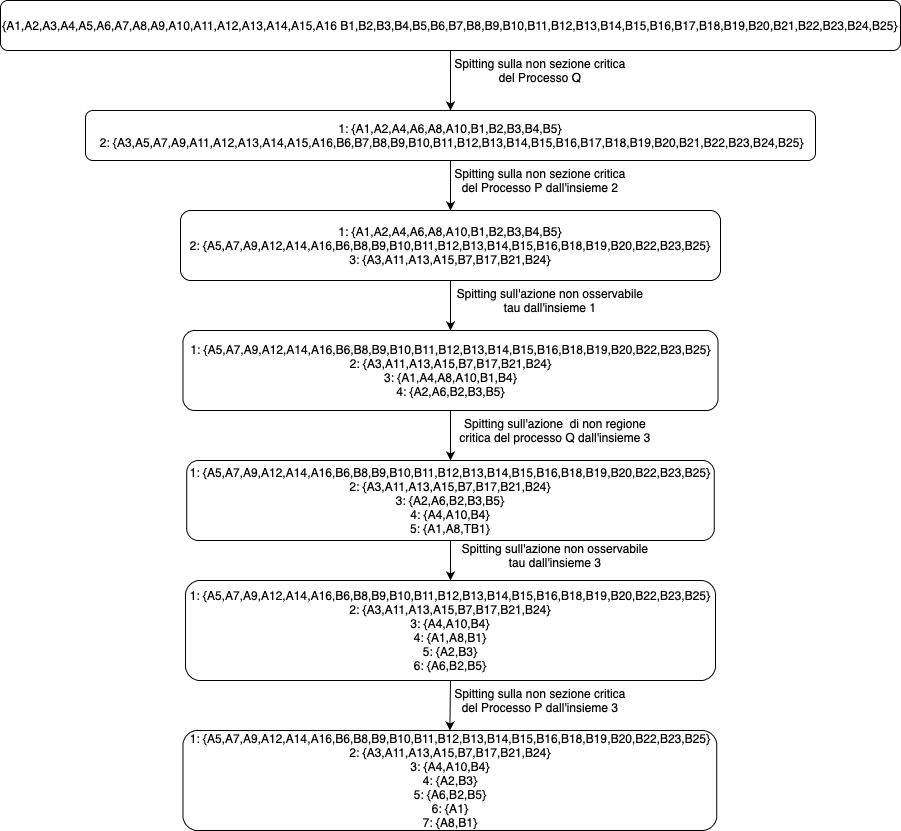
\includegraphics[scale=0.55]{Untitled Diagram-4.png}
\end{figure}
\\Individuati \textit{A1} e \textit{B1} appartenenti a 2 insiemi differenti concludiamo che i processi non sono bisimili.
\clearpage
\section{Algoritmo 3.8}
Analogamente all'algoritmo 3.6, l'Algoritmo 3.8 prevede 2 variabili boolean \textit{wantp} e \textit{wantq} che vengono impostate rispettivamente a \textit{true} nel processo \textit{p} e \textit{q} per poter entrare nella regione critica e al termine al fine di permettere l'esecuzione dell'altro processo settando a \textit{false}. A differenza del precedente, in questo caso si invertono \textit{p2} e \textit{p3} continuando a prevedere che ogni processo, all'inizio della propria esecuzione, possa senza limiti ciclare in sezione non critica bloccando l'altro processo. 
\begin{figure}[h] 
\centering
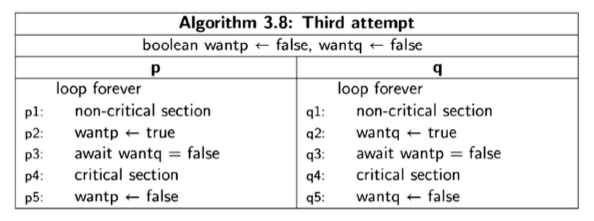
\includegraphics[scale=0.6]{3.8.png}
\end{figure}
\clearpage
\subsection{Rete di Petri}
\begin{figure}[h] 
\centering
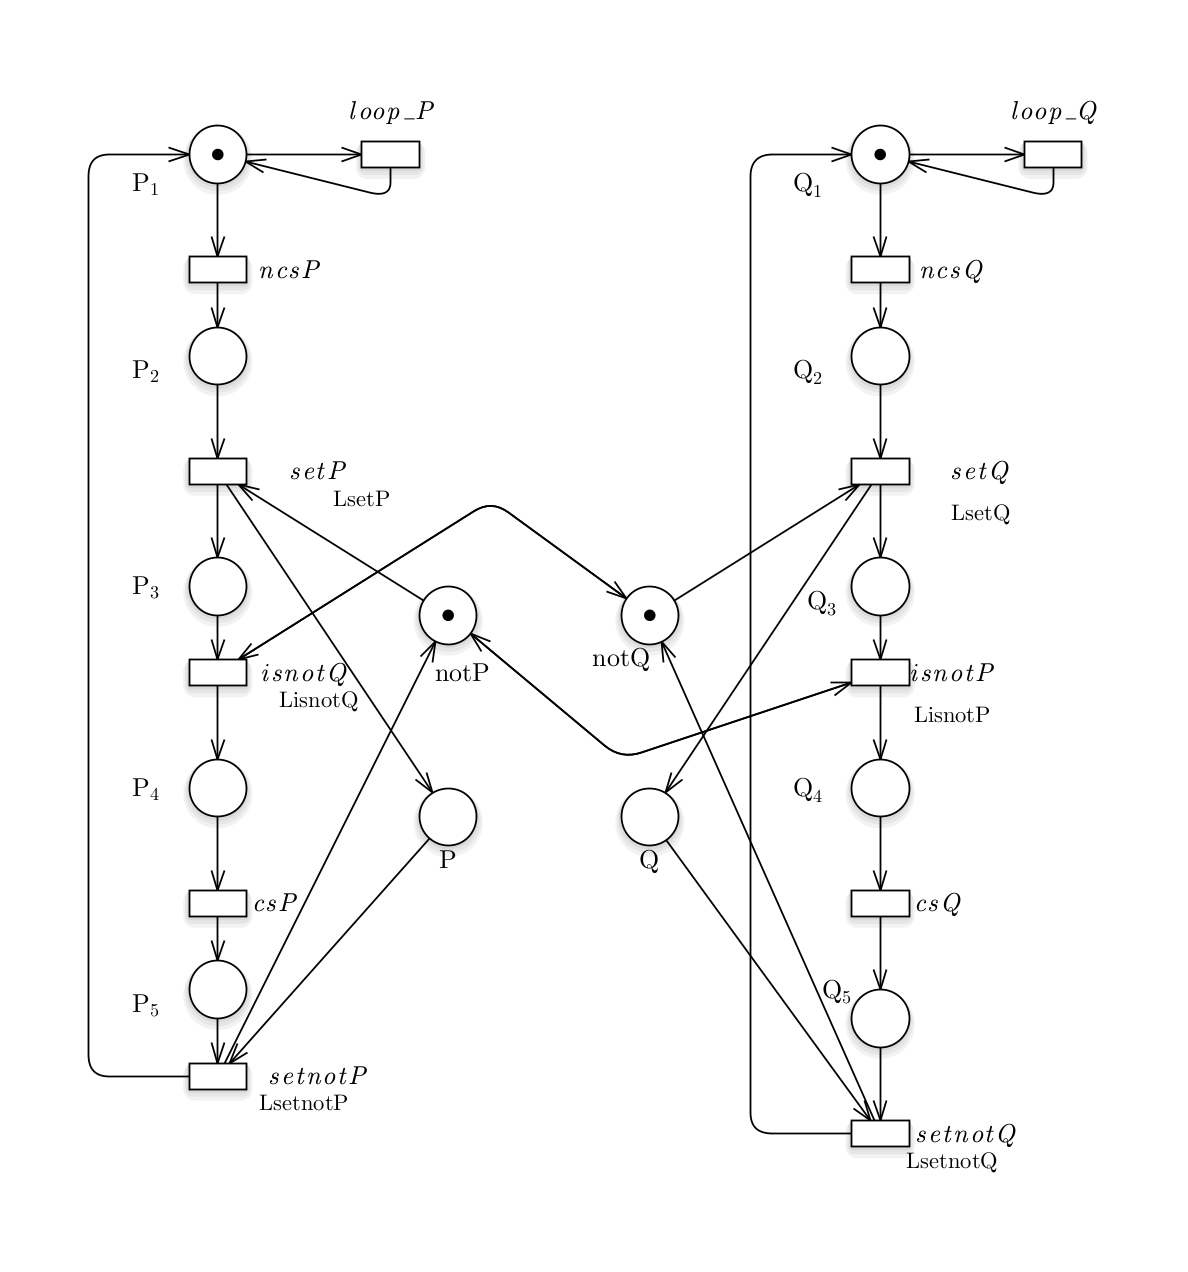
\includegraphics[scale=0.4]{3.8PT.png}
\end{figure}
\subsection{Analisi GreatSPN}
\begin{tabular}{ |p{6cm}||p{3cm}|p{3cm}|}
 \hline
 PROPRIETA'& CTL\\
 \hline
 MUTUA ESCLUSIONE&TRUE \\
 DEADLOCK PROCESSO p&FALSE \\
 DEADLOCK PROCESSO q&FALSE\\
 STARVATION PROCESSO p&FALSE\\
 STARVATION PROCESSO p&FALSE\\
\hline
\end{tabular}
\begin{itemize}
    \item MUTUA ESCLUSIONE: è rispettata in quanto le verifiche sulle variabili \textit{wantp} e \textit{wantq} impedisce che possano accedere in regione critica contemporaneamente .
    \item DEADLOCK: non è rispettato in quanto i processi \textit{p} e \textit{q} potrebbero impostare a TRUE le rispettive variabile impedendo ad entrambi di procedere e inoltre possono ciclare all'infinito in regione non critica (p1 e q1) essendo che non sono obbligati i processi al progresso;
    \item STARVATION: non è rispetta in quanto non c'è assenza di deadlock.
\end{itemize}
\clearpage
\subsection{NuSMV}
L'implementazione dell'algoritmo 3.8 in NuSMV prevede un modulo main in cui si definiscono 2 variabili di tipo boolean impostate entrambe a FALSE \textit{wantp} e \textit{wantq} e 2 processi \textit{p} e \textit{q} e il modulo user che ha come parametri le variabili  \textit{wantp} e \textit{wantq}. 
\\L'algoritmo 3.8 si differenzia dal 3.6 nell'ordine in cui viene eseguita la verifica delle variabili \textit{wantp} e \textit{wantq}.
\\Nel modulo user sono definiti 5 stati in maniera analoga a quanto fatto dall'algoritmo 3.8:
\begin{itemize}
    \item p1 : esecuzione in regione non critica;
    \item p2 : la variabile \textit{wantp} è impostata a TRUE;
    \item p3 : in attesa che la variabile \textit{wantq} sia FALSE;
    \item p4 : esecuzione in regione critica;
    \item p5 : uscita dalla regione critica e variabile \textit{wantp} impostata a FALSE.
\end{itemize}
\begin{figure}[h] 
\centering
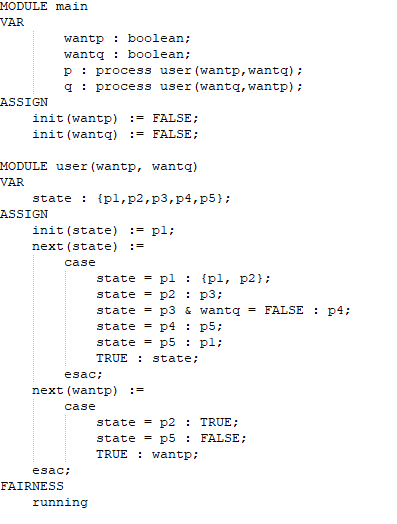
\includegraphics[scale=1.1]{3.8nusmv.png}
\end{figure}
\subsection{Analisi NuSMV LTL}
MUTUA ESCLUSIONE:
\\LTLSPEC
\\G!(p.state = p4 \& q.state = p4)
\\\\DEADLOCK DEL PROCESSO p:
\\LTLSPEC
\\G(p.state = p3 -$>$ F p.state = p4 $|$ q.state = p4)
\\\\DEADLOCK DEL PROCESSO q:
\\LTLSPEC
\\G(q.state = p3 -$>$ F p.state = p4 $|$ q.state = p4)
\\\\STARVATION DEL PROCESSO p:
\\LTLSPEC
\\G(p.state = p3 -$>$ F p.state = p4)
\\\\STARVATION DEL PROCESSO q:
\\LTLSPEC
\\G(q.state = p3 -$>$ F q.state = p4)
\subsection{Analisi NuSMV CTL}
MUTUA ESCLUSIONE
\\SPEC
\\G!(p.state = p4 \& q.state = p4)
\\\\DEADLOCK DEL PROCESSO p:
\\SPEC
\\AG(p.state = p3 -$>$ AF p.state = p4 $|$ q.state = p4)
\\\\DEADLOCK DEL PROCESSO q:
\\SPEC
\\AG(q.state = p3 -$>$ AF p.state = p4 $|$ q.state = p4)
\\\\STARVATION DEL PROCESSO p:
\\SPEC
\\AG(p.state = p3 -$>$ AF p.state = p4)
\\\\STARVATION DEL PROCESSO q:
\\SPEC
\\AG(q.state = p3 -$>$ AF q.state = p4)
\clearpage
\subsection{Analisi Proprietà NuSMV}
\begin{tabular}{|p{6cm}||p{3cm}|p{3cm}|}
\hline
PROPRIETA' & LTL & CTL\\
\hline
 MUTUA ESCLUSIONE&TRUE&TRUE \\
 DEADLOCK PROCESSO p&FALSE&FALSE\\
 DEADLOCK PROCESSO q&FALSE&FALSE\\
 STARVATION PROCESSO p&FALSE&FALSE\\
 STARVATION PROCESSO p&FALSE&FALSE\\
\hline
\end{tabular}
\begin{itemize}
    \item MUTUA ESCLUSIONE: è rispettata in quanto la verifica che la variabile booleana dell'altro processo sia impostata a false limita l'accesso in regione critica ad un solo processo;
    \item DEADLOCK: non è rispettata, come evidenziato dai contro esampi forniti da NuSMV, dato che se entrambi i processi dovessero impostare a true la propria variabile e mettersi in attesa che la variabile dell'altro processo sia settata a false impendendo perciò di procedere in regione critica;
    \item STARVATION: non è rispettata dato che è presente deadlock.
\end{itemize}
\subsection{Riduzione Rete di Petri Algoritmo 3.6}
Per ottenere la Riduzione della rete di Petri si utilizzano le seguenti regole: \textit{RA2} per l'unione dei posti P4,P5 e Q4,Q5;  \textit{RA1} per l'unione delle transizioni ncsP, isnotP per il processo p e ncsQ e isnotQ per il processo Q, infine \textit{RC1} per eliminare il self loop (che permette di non progredire) loop\_P e loop\_Q.
\begin{figure}[h] 
\centering
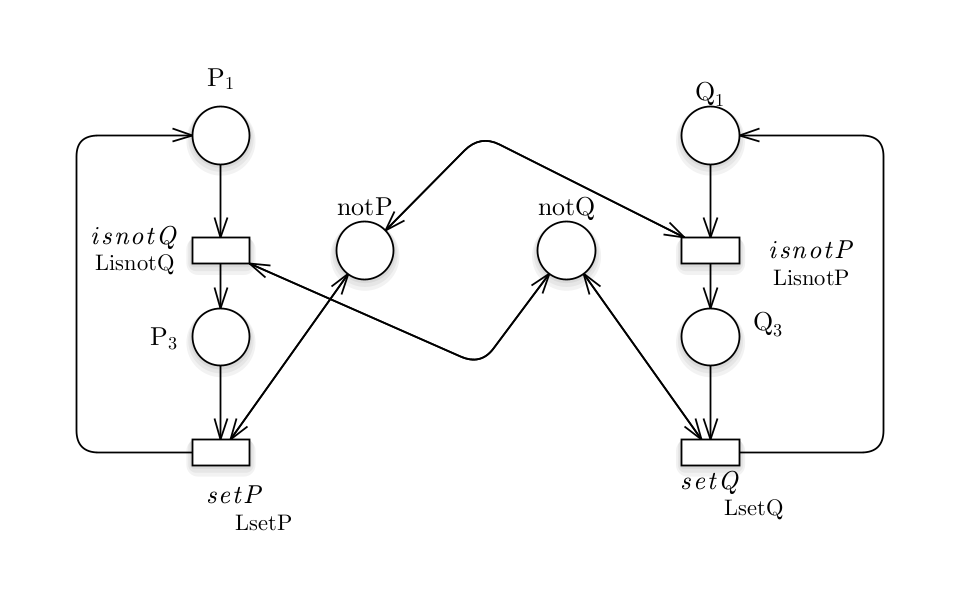
\includegraphics[scale=0.5]{Riduzione3.6.png}
\end{figure}
\clearpage
\subsection{Riduzione Rete di Petri Algoritmo 3.8}
Per ottenere la Riduzione della rete di Petri si utilizzano le seguenti regole: \textit{RA2} per l'unione dei posti P1,P2 e Q1,Q2 e i posti P4,P5 e Q4,Q5, infine \textit{RC1} per eliminare il self loop (che permette di non progredire) loop\_P e loop\_Q.
\begin{figure}[h] 
\centering
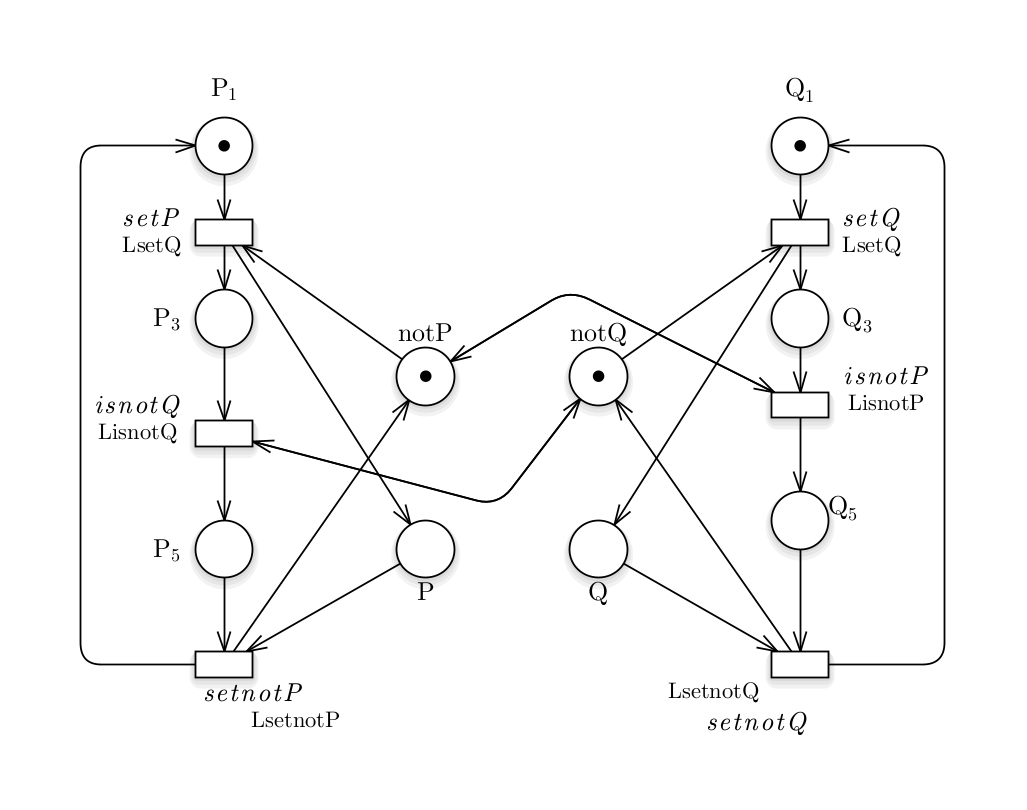
\includegraphics[scale=0.5]{Riduzione3-8.png}
\end{figure}
\clearpage
\subsection{Confronto in Bisimulazione Algoritmo 3.6 e Algoritmo 3.8}
\begin{figure}[h] 
\centering
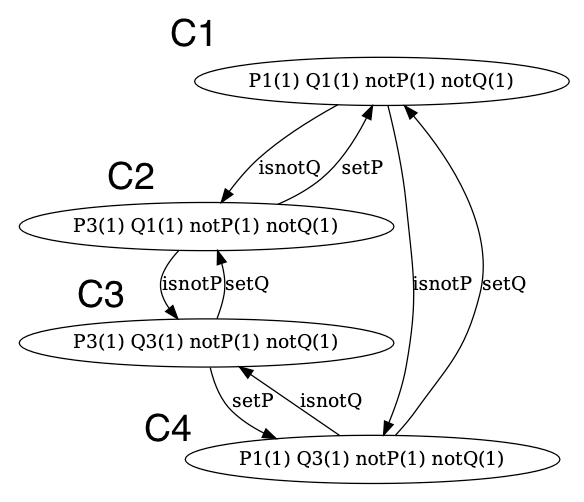
\includegraphics[scale=0.36]{BIS3.6.png}
\end{figure}
\begin{figure}[h] 
\centering
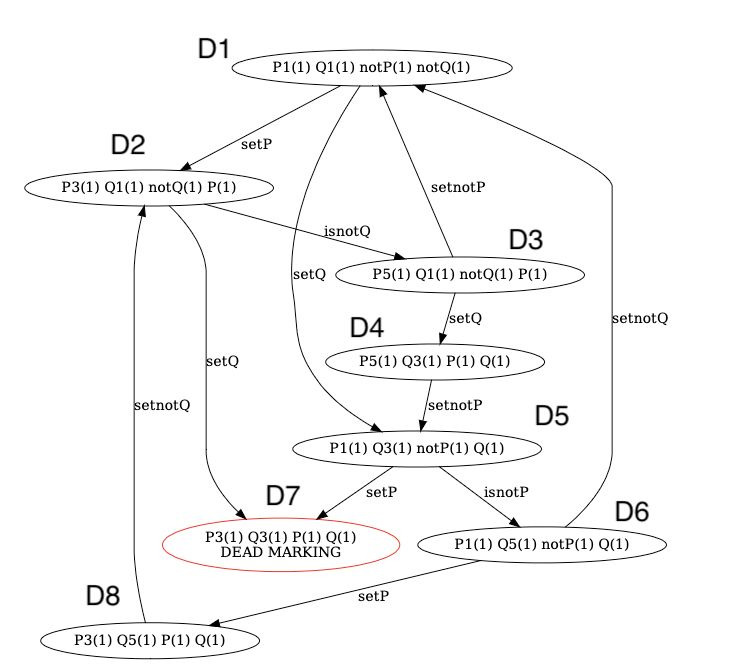
\includegraphics[scale=0.36]{Bis3-8.png}
\end{figure}
Individuati \textit{C1} e \textit{D1} appartenenti a 2 insiemi differenti concludiamo che i processi non sono bisimili.
\begin{figure}[h] 
\centering
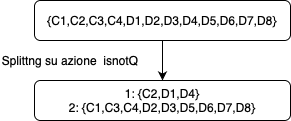
\includegraphics[scale=0.5]{Untitled Diagram-5.png}
\end{figure}
\clearpage
\section{Algoritmo 3.9}
L'Algoritmo 3.9 prevede 2 variabili boolean \textit{wantp} e \textit{wantq} che vengono impostate rispettivamente a \textit{true} nel processo \textit{p} e \textit{q} e successivamente entrano nel loop in attesa che la variabile dell'altro processo sia settata a FALSE per poter entrare nella regione critica e al termine al fine di permettere l'esecuzione dell'altro processo settando a \textit{false}. Viene inserito un ciclo while per garantire la mutua esclusione e inoltre all'inizio della propria esecuzione i processi possono senza limiti ciclare in sezione non critica bloccando l'altro processo. 
\begin{figure}[h] 
\centering
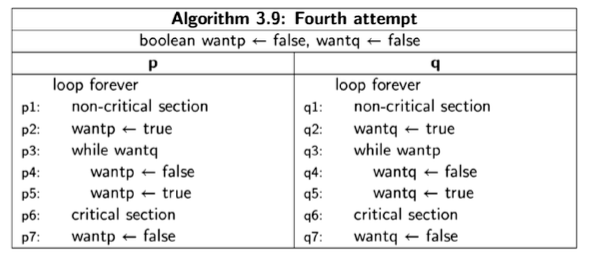
\includegraphics[scale=0.6]{3.9.png}
\end{figure}
\clearpage
\subsection{Rete di Petri}
\begin{figure}[h] 
\centering
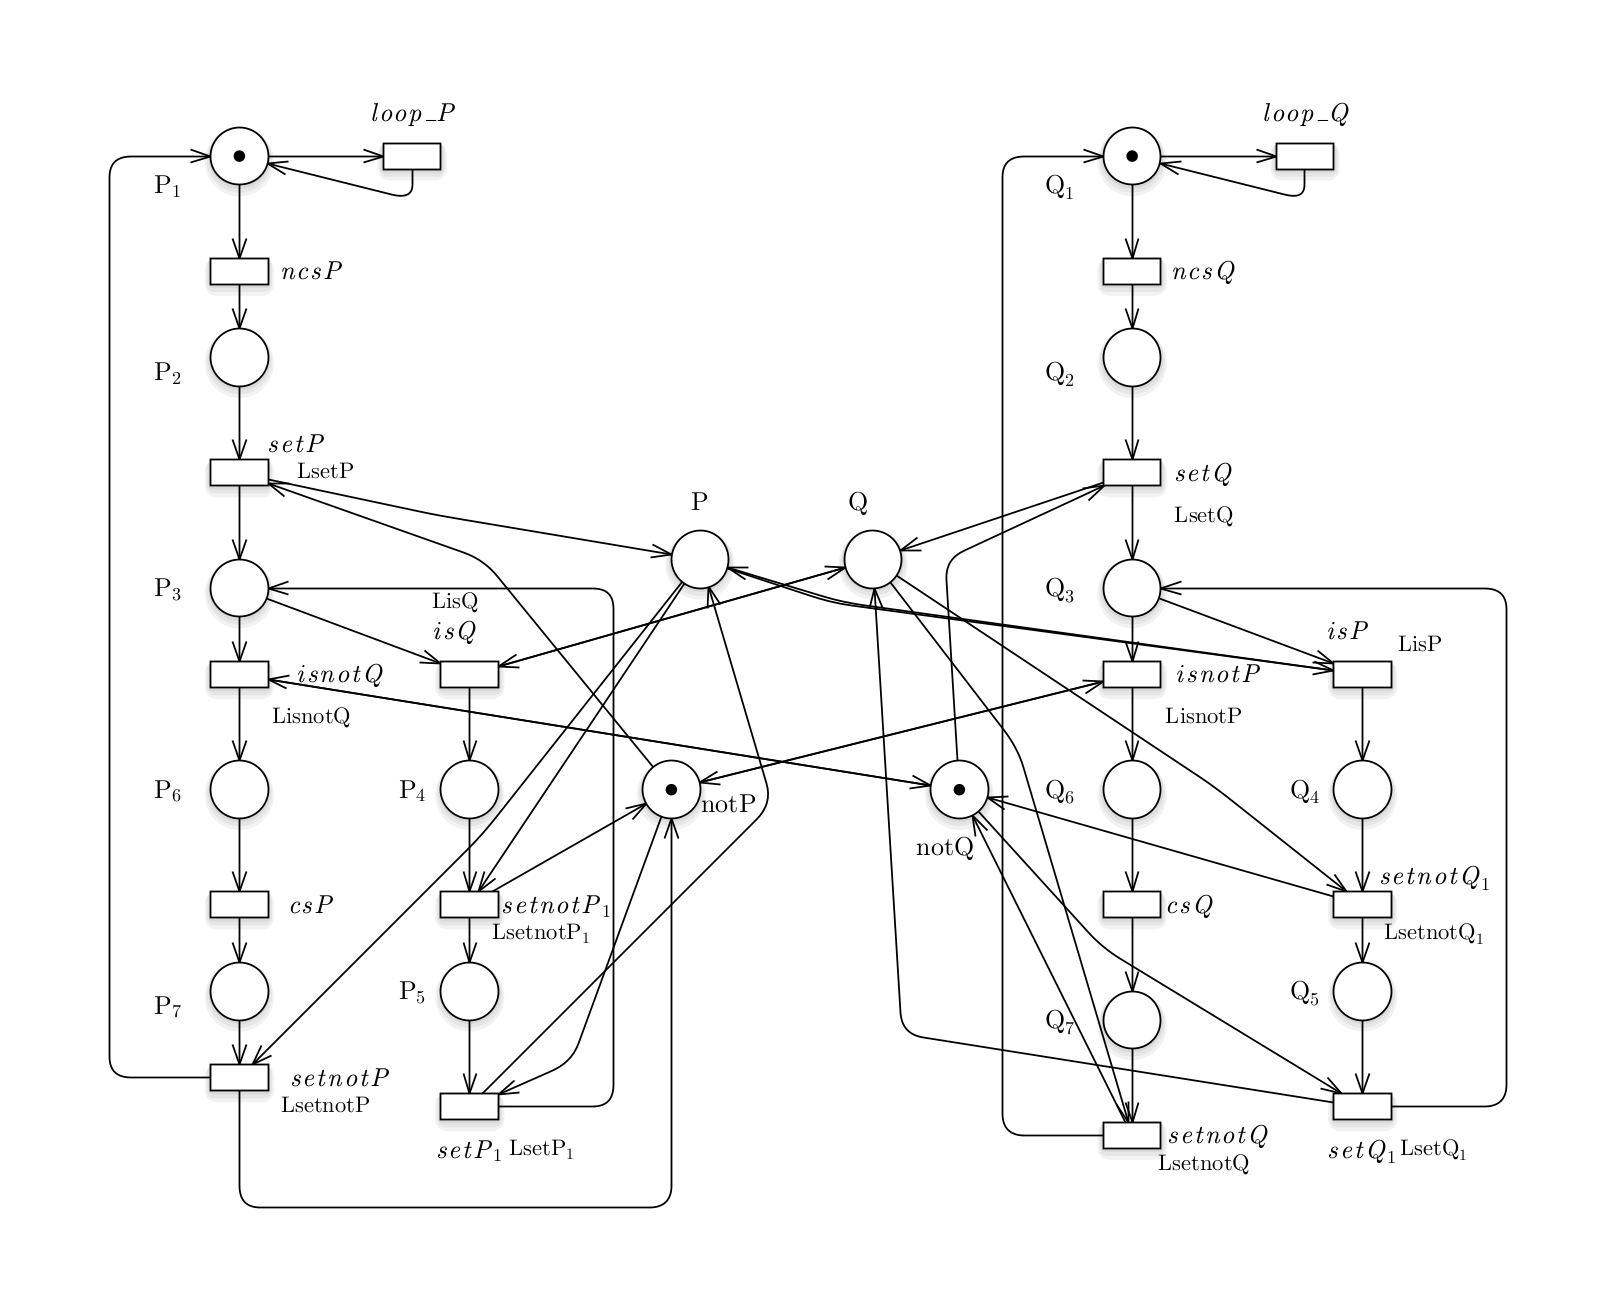
\includegraphics[scale=0.3]{3.9PT.png}
\end{figure}
\subsection{Analisi GreatSPN}
\begin{tabular}{ |p{6cm}||p{3cm}|p{3cm}|}
 \hline
 PROPRIETA'& CTL\\
 \hline
 MUTUA ESCLUSIONE&TRUE \\
 DEADLOCK PROCESSO p&FALSE \\
 DEADLOCK PROCESSO q&FALSE\\
 STARVATION PROCESSO p&FALSE\\
 STARVATION PROCESSO p&FALSE\\
\hline
\end{tabular}
\begin{itemize}
    \item MUTUA ESCLUSIONE: è rispettata in quanto le verifiche effettuate sulle variabili \textit{wantp} e \textit{wantq}, condivisa da entrambi i processi, impedendo che possano accedere in regione critica contemporaneamente.
    \item DEADLOCK: non è rispettata in quanto le verifiche all'interno del loop potrebbero non far progredire entrambi i processi, inoltre possono ciclare all'infinito in regione non critica (p1 e q1) essendo che non sono obbligati al progresso;
    \item STARVATION: non è rispetta in quanto non c'è assenza di deadlock.
\end{itemize}
\clearpage
\subsection{NuSMV}
L'implementazione dell'algoritmo 3.9 in NuSMV prevede un modulo main in cui si definisce una variabile globale \textit{turn} e 2 processi \textit{p} e \textit{q} mediante il modulo user che ha come parametri la stessa variabile \textit{turn} e 2 valori che rappresentano rispettivamente il valore della variabile turn rispetto al processo in esecuzione. 
\\Nel modulo user sono definiti 4 stati in maniera analoga a quanto fatto dall'algoritmo 3.2:

\begin{itemize}
    \item p1 : esecuzione in regione non critica;
    \item p2 : la variabile \textit{wantp} è impostata a TRUE;
    \item p3 : in attesa che la variabile \textit{wantq} sia TRUE;
    \item p4 : la variabile \textit{wantp} è impostata a FALSE;
    \item p5 : la variabile \textit{wantp} è impostata a TRUE;
    \item p6 : esecuzione in regione critica;
    \item p7 : uscita dalla regione critica e variabile \textit{wantp} impostata a FALSE.
\end{itemize}
\begin{figure}[h] 
\centering
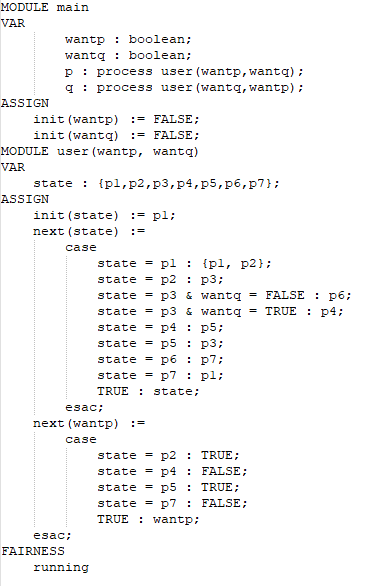
\includegraphics[scale=0.95]{3.9nusmv.png}
\end{figure}
\subsection{Analisi NuSMV LTL}
MUTUA ESCLUSIONE:
\\LTLSPEC
\\G!(p.state = p6 \& q.state = p6)
\\\\DEADLOCK DEL PROCESSO p:
\\LTLSPEC
\\G(p.state = p2 -$>$ F p.state = p6 $|$ q.state = p6)
\\\\DEADLOCK DEL PROCESSO q:
\\LTLSPEC
\\G(q.state = p2 -$>$ F p.state = p6 $|$ q.state = p6)
\\\\STARVATION DEL PROCESSO p:
\\LTLSPEC
\\G(p.state = p2 -$>$ F p.state = p6)
\\\\STARVATION DEL PROCESSO q:
\\LTLSPEC
\\G(q.state = p2 -$>$ F q.state = p6)
\subsection{Analisi NuSMV CTL}
MUTUA ESCLUSIONE
\\SPEC
\\G!(p.state = p6 \& q.state = p6)
\\\\DEADLOCK DEL PROCESSO p:
\\SPEC
\\AG(p.state = p2 -$>$ AF p.state = p6 $|$ q.state = p6)
\\\\DEADLOCK DEL PROCESSO q:
\\SPEC
\\AG(q.state = p2 -$>$ AF p.state = p6 $|$ q.state = p6)
\\\\STARVATION DEL PROCESSO p:
\\SPEC
\\AG(p.state = p2 -$>$ AF p.state = p6)
\\\\STARVATION DEL PROCESSO q:
\\SPEC
\\AG(q.state = p2 -$>$ AF q.state = p6)
\subsection{Analisi Proprietà NuSMV}
\begin{tabular}{|p{6cm}||p{3cm}|p{3cm}|}
\hline
PROPRIETA' & LTL & CTL\\
\hline
 MUTUA ESCLUSIONE&TRUE&TRUE \\
 DEADLOCK PROCESSO p&FALSE&FALSE\\
 DEADLOCK PROCESSO q&FALSE&FALSE\\
 STARVATION PROCESSO p&FALSE&FALSE\\
 STARVATION PROCESSO p&FALSE&FALSE\\
\hline
\end{tabular}
\begin{itemize}
    \item MUTUA ESCLUSIONE: è rispettata in quanto le verifiche effettuate sulle variabili \textit{wantp} e \textit{wantq}, condivisa da entrambi i processi, impedendo che possano accedere in regione critica contemporaneamente;
    \item DEADLOCK: non è rispettata, come evidenziato dai contro esampi forniti da NuSMV, dato che se entrambi i processi dovessero trovarsi nello stato p3, in cui verificano che la variabile condivisa dell'altro processo sia false, ripetendo il ciclo infinite volte dato che la condizione non sarà mai verificata;
    \item STARVATION: non è rispettata dato che è presente deadlock.
\end{itemize}
\clearpage
\section{Algoritmo 3.10}
L'algoritmo 3.10 include al suo interno sia le variabili boolean \textit{wantp} e \textit{wantq} e anche \textit{turn}.
\begin{figure}[h] 
\centering
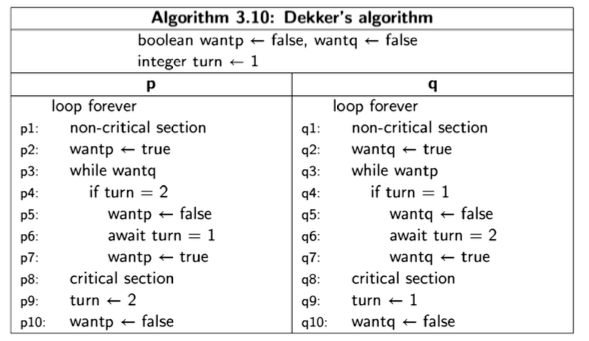
\includegraphics[scale=0.6]{3.10.png}
\end{figure}
\clearpage
\subsection{Rete di Petri}
\begin{figure}[h] 
\centering
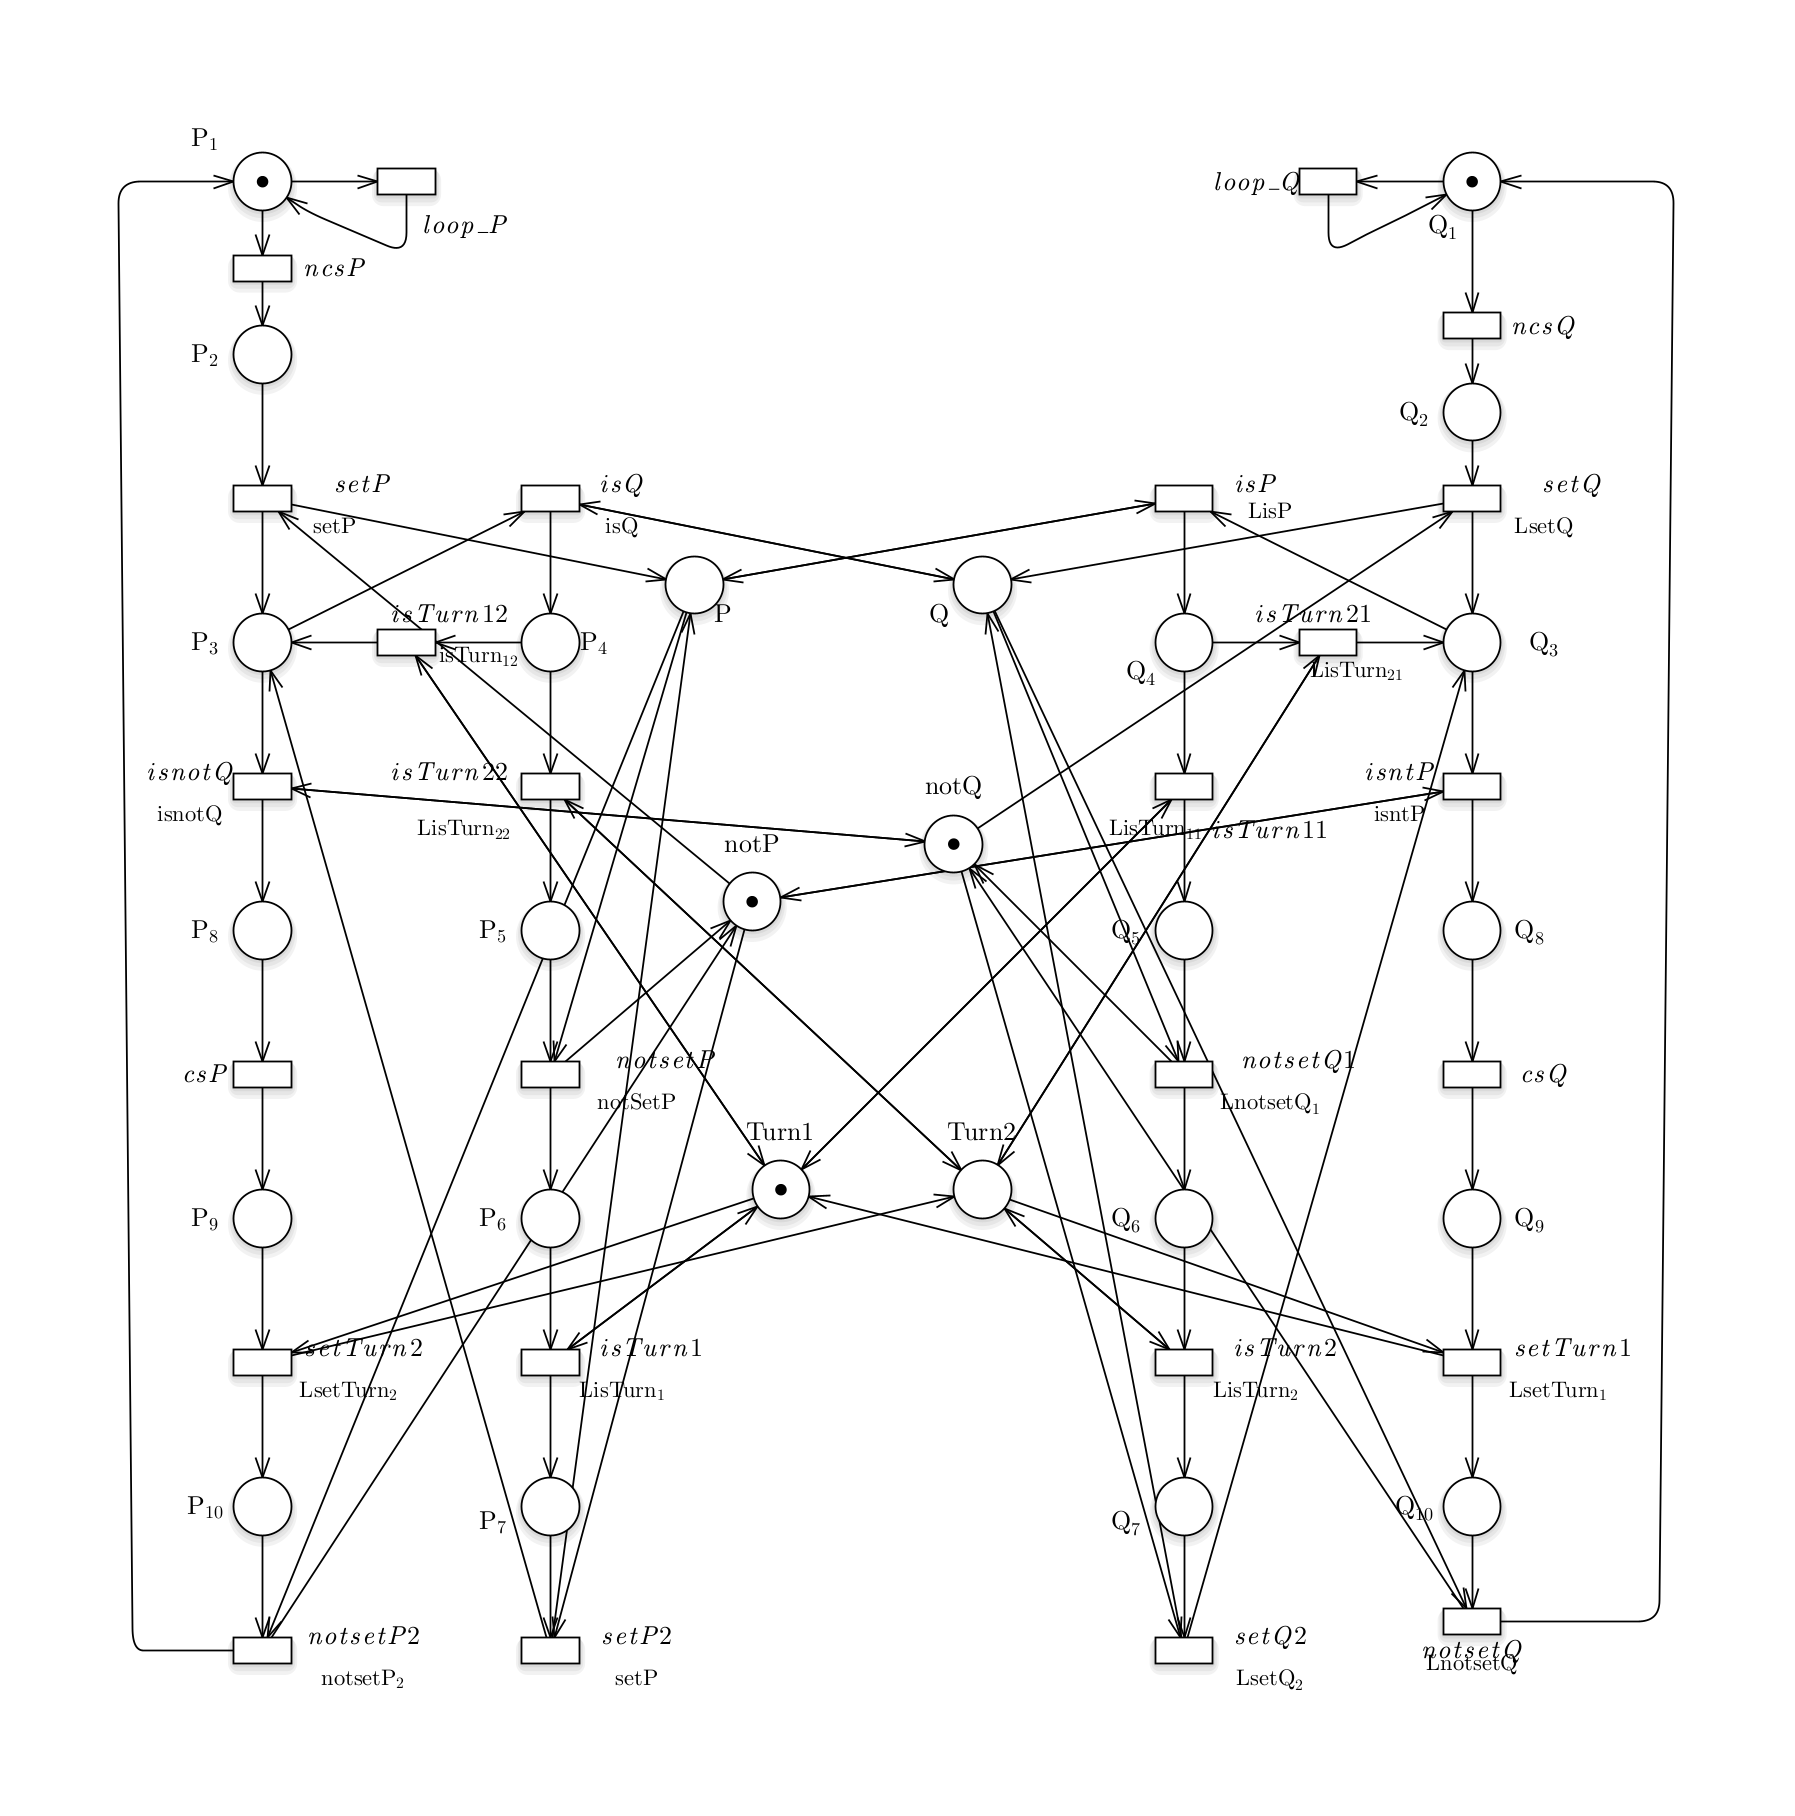
\includegraphics[scale=0.29]{3.10PT.png}
\end{figure}
\subsection{Analisi GreatSPN}
\begin{tabular}{ |p{6cm}||p{3cm}|p{3cm}|}
 \hline
 PROPRIETA'& CTL\\
 \hline
 MUTUA ESCLUSIONE&TRUE \\
 DEADLOCK PROCESSO p&FALSE \\
 DEADLOCK PROCESSO q&FALSE\\
 STARVATION PROCESSO p&FALSE\\
 STARVATION PROCESSO p&FALSE\\
\hline
\end{tabular}
\begin{itemize}
    \item MUTUA ESCLUSIONE: è rispettata in quanto la variabile turn, condivisa da entrambi i processi, impedisce che possano accedere in regione critica contemporaneamente .
    \item DEADLOCK: non è rispettato in quanto i processi posso ciclare all'infinito in regione non critica (p1 e q1) essendo che non sono obbligati al progresso;
    \item STARVATION: non è rispettata in quanto non c'è assenza di deadlock.
\end{itemize}
\clearpage
\subsection{NuSMV}
L'implementazione dell'algoritmo 3.9 in NuSMV prevede un modulo main in cui si definisce una variabile globale \textit{turn} e 2 processi \textit{p} e \textit{q} mediante il modulo user che ha come parametri la stessa variabile \textit{turn} e 2 valori che rappresentano rispettivamente il valore della variabile turn rispetto al processo in esecuzione. 
\\Nel modulo user sono definiti 4 stati in maniera analoga a quanto fatto dall'algoritmo 3.2:

\begin{itemize}
    \item p1 : esecuzione in regione non critica;
    \item p2 : la variabile \textit{wantp} è impostata a TRUE;
    \item p3 : in attesa che la varibaile \textit{wantq} sia TRUE;
    \item p4 : in attesa che la variabile \textit{turn} sia otherproc;
    \item p5 : la variabile \textit{wantp} è impostata a FALSE;
    \item p6 : in attesa che la variabile \textit{turn} sia myproc;
    \item p7 : la variabile \textit{wantp} è impostata a TRUE;
    \item p8 : esecuzione in regione critica;
    \item p9 : la variabile \textit{turn} è impostata a otherproc;
    \item p10: uscita dalla regione critica e variabile \textit{wantp} impostata a FALSE.
\end{itemize}
\begin{figure}[h] 
\centering
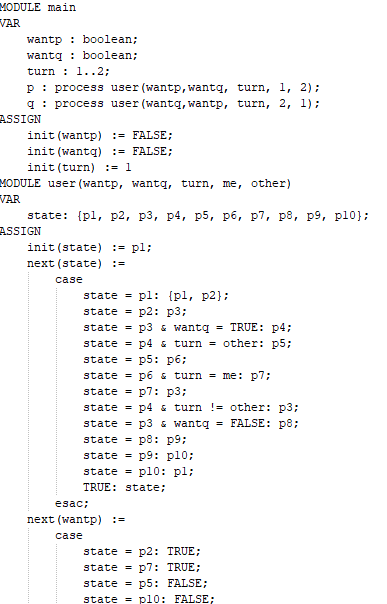
\includegraphics[scale=0.8]{3.10nusmv.png}
\end{figure}
\begin{figure}[h] 
\centering
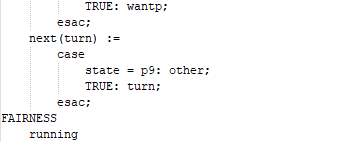
\includegraphics[scale=0.8]{3.101nusmv.png}
\end{figure}
\subsection{Analisi NuSMV LTL}
MUTUA ESCLUSIONE:
\\LTLSPEC
\\G!(p.state = p8 \& q.state = p8)
\\\\DEADLOCK DEL PROCESSO p:
\\LTLSPEC
\\G(p.state = p2 -$>$ F p.state = p8 $|$ q.state = p8)
\\\\DEADLOCK DEL PROCESSO q:
\\LTLSPEC
\\G(q.state = p2 -$>$ F p.state = p8 $|$ q.state = p8)
\\\\STARVATION DEL PROCESSO p:
\\LTLSPEC
\\G(p.state = p2 -$>$ F p.state = p8)
\\\\STARVATION DEL PROCESSO q:
\\LTLSPEC
\\G(q.state = p2 -$>$ F q.state = p8)
\subsection{Analisi NuSMV CTL}
MUTUA ESCLUSIONE
\\SPEC
\\G!(p.state = p8 \& q.state = p8)
\\\\DEADLOCK DEL PROCESSO p:
\\SPEC
\\AG(p.state = p2 -$>$ AF p.state = p8 $|$ q.state = p8)
\\\\DEADLOCK DEL PROCESSO q:
\\SPEC
\\AG(q.state = p2 -$>$ AF p.state = p8 $|$ q.state = p8)
\\\\STARVATION DEL PROCESSO p:
\\SPEC
\\AG(p.state = p2 -$>$ AF p.state = p8)
\\\\STARVATION DEL PROCESSO q:
\\SPEC
\\AG(q.state = p2 -$>$ AF q.state = p8)
\subsection{Analisi Proprietà NuSMV}
\begin{tabular}{|p{6cm}||p{3cm}|p{3cm}|}
\hline
PROPRIETA' & LTL & CTL\\
\hline
 MUTUA ESCLUSIONE&TRUE&TRUE \\
 DEADLOCK PROCESSO p&TRUE&TRUE\\
 DEADLOCK PROCESSO q&TRUE&TRUE\\
 STARVATION PROCESSO p&TRUE&TRUE\\
 STARVATION PROCESSO p&TRUE&TRUE\\
\hline
\end{tabular}
\begin{itemize}
    \item MUTUA ESCLUSIONE: è rispettata;
    \item DEADLOCK: è rispettata;
    \item STARVATION: è rispettata.
\end{itemize}
\subsection{Progresso solo in regione critica}
Si richiede di verificare le conseguenze di progresso solo in regione critica ma non nel protocollo di accesso e pertanto il processo potrà rimanere fermo per un tempo indefinito invece di accedere in regione critica. Per implementare questa versione dell'Algoritmo in NuSMV è sufficiente permettere al processo di poter non proseguire quando si trova in p4. Viene riportata la modifica rispetto all'implementazione della versione orginiale.
\begin{figure}[h] 
\centering

\includegraphics[scale=1]{versionediversa.png}
\end{figure}

\subsection{Analisi Proprietà NuSMV}
\begin{tabular}{|p{6cm}||p{3cm}|p{3cm}|}
\hline
PROPRIETA' & LTL & CTL\\
\hline
 MUTUA ESCLUSIONE&TRUE&TRUE \\
 DEADLOCK PROCESSO p&FALSE&FALSE\\
 DEADLOCK PROCESSO q&FALSE&FALSE\\
 STARVATION PROCESSO p&FALSE&FALSE\\
 STARVATION PROCESSO p&FALSE&FALSE\\
\hline
\end{tabular}
\begin{itemize}
    \item MUTUA ESCLUSIONE: è rispettata;
    \item DEADLOCK: non è rispettata dato che che i processi possono non progredire rimanendo in \textit{p4};
    \item STARVATION: non è rispettata in quanto non c'è assenza di deadlock..
\end{itemize}
\end{document}
